\chapter[Lecture 25]{}\label{lec25}
\begin{figure}[H]
\centering
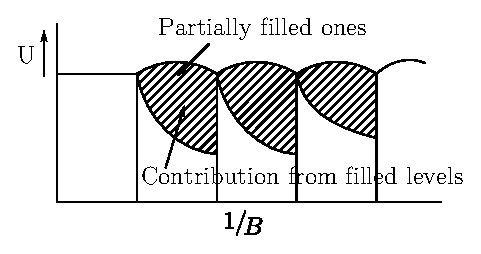
\includegraphics{images/lecture25/fig14.eps}
\end{figure}

$\mu=-\dfrac{\partial U}{\partial B}$ Oscillates as a function of $\dfrac{1}{B}$ called $dH_{v}A$ oscillation.

The interval of oscillation $\Delta\left(\dfrac{1}{B}\right)=\dfrac{2\pi e}{\hbar \subset S}$

$S\to$ Extremal area of Fermi surface normal to $\overrightarrow{B}$.
\begin{figure}[H]
\centering
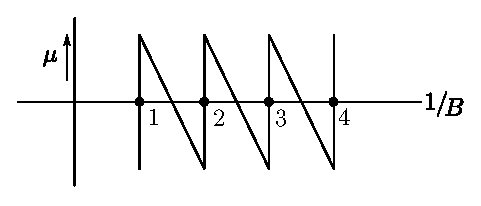
\includegraphics{images/lecture25/fig15.eps}
\end{figure}

\section*{Direct method - ARPES}

Discovery of electrons J.J. Thomson - 1897.

Drude (1900) put forward his theory of metallic conduction.

Solid consists of heavy (+ve) charge (immobile) and mobile electrons that makes them neutral solid.

Some fraction of electrons of $z$ electrons ($z=$ atomic no.) are strongly attached to (+ve) charge $\to$ don't move much that rest moves all over the solid and can be treated like classical electron gas, with velocity distance following Maxwell- Boltzmann Distance.
$$
f_{2}=n\left(\dfrac{m}{2\pi k_{B^{T}}}\right)^{\frac{3}{2}}e^{-m\nu^{2}/2k_{B^{T}}}
$$

This worked quite well $\to$ Wiedemann - Franz law.

Specific heat $\dfrac{3}{2}k_{B}$ per electron $\to$ this was not observed.

Later after Quantum theory came, Pauli's exclussion principle needs to be applied and Fermi-Dirac Distribution $\to$ {\em Sommerfeld's model.}

\section*{Free-electron approximation}

\subsection*{Drude's model}

\subsection*{Heat Capacity}
$$
e_{F}\sim k_{B}T_{F}\quad T_{F}\sim 10^{4}K
$$
$\therefore \ \dfrac{T}{T_{F}}$ is very small close to room temperature.

$\therefore$ The fraction of electrons taking part in heat capacity is $\sim \dfrac{T}{T_{F}}$
\begin{gather*}
\therefore \ U_{el}=\left(N\dfrac{T}{T_{F}}\right)K_{B}T\quad N= \text{ total no. of electrons.}\\
\therefore \ C_{el}=\dfrac{\partial U_{el}}{\partial T}\simeq N k_{B}T/T_{F}=\gamma T\\
\gamma \text{ is a const } \to \text{ measure of effective mass.}\\
\therefore \ \fbox{$C=\gamma T+AT^{3}$}\quad T^{3} \text{ is phonon part.}
\end{gather*}
at plot of $C/T$ with $T^{2}$ given $\gamma$ and $A$, and we can measure effective mass that way, $\gamma\to$ measure of effective mass.

A factor $\dfrac{\pi^{2}}{2}$ appears if calculated using Formi-Dirac distribution.

\section*{Force on an electron}
$$
F=-e(\overrightarrow{E}+\dfrac{1}{e}\overrightarrow{\nu}\times \overrightarrow{B})
$$
In an electric field
$$
\delta k=-\dfrac{eEt}{\hbar}\quad \nu=-\dfrac{eE\tau}{m}\Leftarrow m\nu=\hbar k
$$

Due to scattering of electrons, $t\sim \tau\to$ relaxation [The electric field acts till the electron gets scattered] time.
\begin{gather*}
\therefore\quad J=nq\overrightarrow{\nu}=ne^{2}\tau E/m\\
\therefore\quad \sigma =\dfrac{j}{E}=\dfrac{ne^{2}\tau}{m}\quad \rho=\dfrac{1}{r}=\text{ resistivity.}
\end{gather*}

Scattering can be due to phonons $(\tau_{i})$ or impurities $(\tau_{i})$
$$
\dfrac{1}{\widetilde{L}}=\dfrac{1}{\widetilde{L}_{L}}+\dfrac{1}{\widetilde{L}_{i}}\quad \text{Marthiessen's rule.}
$$
$\rho(T)/\rho(0)=$ residual resistivity ratio.

Impurity scattering usually independent of temperature $T$.

Phonon contribution is dependent on no. of phonons at a particular temperature $T$ usually \fbox{$\rho_{L}\alpha T$}.

\section*{Umklapp Scattering}
\begin{figure}[H]
\centering
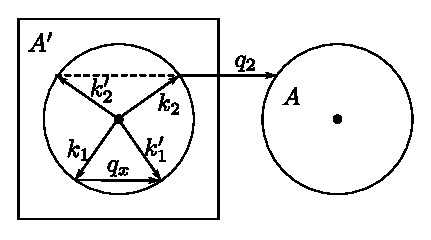
\includegraphics{images/lecture25/fig1.eps}
\end{figure}

Scattering $\to$
$$
k'_{1}=k_{1}+q_{1}
$$
If this scattering involves a reciprocal lattice vector, it is called Umklapp scattering. e.g.,
$$
k'_{2}=k_{2}+q_{2}\pm G
$$
\begin{itemize}
\itemsep=0pt
\item a scattering of electron with wave vector $k_{2}$, results to a final wave vector $k'_{2}$ which involves lattice translation $G=AA'$.

\item The angle of scattering is large $\to \sim \pi$ strong scatterers.

\item If the Fermi surface does not intersect zone boundary, one needs minimum value of $q(=q_{0})$ to have Umklapp scattering.

\item At low temperature, Umklapp scattering goes as $e^{-\theta_{U}/T}$

$\theta_{U}=$ Characteristic temperature

For potassium $\theta_{U}=23K$\quad $\theta_{D}=91K$

$\therefore$ at low temperature, Umklapp scattering is almost {\em zero}.
\end{itemize}
$\therefore$ Resistivity is dominated by small angle scattering.

\section*{Motion in Magnetic field}

Force on an electron $=F=\dfrac{dp}{dt}=\dfrac{\hbar dk}{dt}\quad P=\hbar k$

However, due to scattering, the fermi sphere will experience a friction at a rate $\dfrac{1}{\tau}$
$$
\therefore \ F=\hbar \left(\dfrac{d}{dt}+\dfrac{1}{\tau}\right)\delta k
$$
change in Momentum + Friction.
$$
\therefore\quad \hbar \dfrac{dk}{dt}+\dfrac{1}{\tau}\hbar \delta k=-e\left[\overrightarrow{E}+\dfrac{1}{C}\overrightarrow{\nu}\times \overrightarrow{B}\right] \text{ (Lorenz force)}
$$
if $\overrightarrow{B}=B\widehat{z}$.
\begin{align*}
m\left(\dfrac{d\nu_{x}}{dt}\right)+\dfrac{v_{n}}{\tau} &= -e\left(E_{x}+\dfrac{B}{C}\nu_{y}\right)\\[3pt]
m\dfrac{d\nu_{y}}{dt}+\dfrac{\nu_{y}}{\tau} &= -e\left(E_{y}-\dfrac{B}{C}\nu_{x}\right)\\
m\dfrac{d\nu_{z}}{dt}+\dfrac{\nu_{z}}{\tau} &= -eE_{z}
\end{align*}
In the steady state in a static electric field, derivatives are zero.
\begin{gather*}
\therefore\quad 
\fbox{
$
\begin{array}{l}
\nu_{x}=-\dfrac{e\tau}{m}E_{x}-w_{C}\tau \nu_{y}\\
\nu_{y}=-\dfrac{e\tau}{m}E_{y}+w_{C}\tau \nu_{x}\\
\nu_{z}=-\dfrac{e\tau}{m}E_{z}
\end{array}
$
}\\
w_{C}=\dfrac{eB}{m_{C}}=\text{ cyclotron frequency}
\end{gather*}
$w_{C}\tau$ is (cyclotron frequency multiplied by time) and an important number.

$w_{C}\tau$ is unity of larger, the effect of magnetic field on electron orbits is significant.

\section*{Hall effect}

Electric field developed across two faces of a conductor in the direction $\overrightarrow{j}\times \overrightarrow{B}$

If $\overrightarrow{J}=J\widehat{x}$; $\overrightarrow{B}=B\widehat{z}$
\begin{figure}[H]
\centering
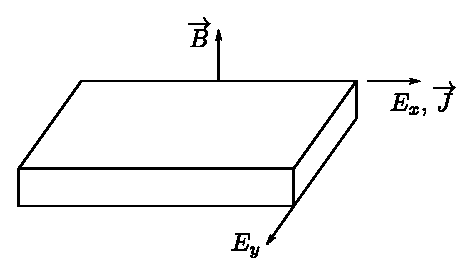
\includegraphics{images/lecture25/fig2.eps}
\end{figure}

Then $\delta \nu_{y}=0$ as current is not flowing out in $y$ direction
$$
\therefore \ E_{y}=\dfrac{w_{C}m}{e}\nu_{x}=-w_{C}\tau E_{x}=-\dfrac{eB\tau}{m_{C}}\cdot E_{x}.
$$

The quantity $\dfrac{E_{y}}{J_{x}B}$ is called Hall co-efficient $R_{H}$.
\begin{gather*}
\therefore \ R_{H} = \left. -\dfrac{eB\tau E_{\lambda}/m_{C}}{ne^{2}\tau E_{x}B/m}=-\dfrac{1}{neC}\right| J=\dfrac{ne^{2}\tau E_{x}}{m}\\[7pt]
\therefore \ \fbox{$R_{H}=-\dfrac{1}{neC}$}\quad\text{or}\quad \fbox{$R_{H}=-\dfrac{1}{ne}$}\quad \text{SI unit.}
\end{gather*}
(-ve) for free electrons. $e$ is magnitude of electrons charge.
\begin{itemize}
\item[(i)] Get carrier concentration

\item[(ii)] Type of carriers.
\end{itemize}
Assumption, all relaxation times are equal.

If both electrons and holes conduct, the scenario is complex.

\section*{Thermal Conductivity of Metals}
$$
J_{Q}=-K\dfrac{dT}{dx}
$$
\begin{align*}
K &= \text{ thermal conductivity}\\
 &= \frac{1}{3}C\nu l
\end{align*}
\begin{quote}
$C$ = heat capacity

$\nu$ = Drift velocity (Avg. velocity)

$l$ = mean free path.
\end{quote}
\begin{align*}
C_{el} &= \frac{\pi^{2}}{2}Nk_{B}T/T_{F}\\
\epsilon_{F} &= k_{B}T_{F}=\frac{1}{2}m\nu^{2}_{F}
\end{align*}
\begin{align*}
\therefore\quad K_{el}=\frac{1}{3}\cdot \frac{\pi^{2}}{2}k_{B}T\cdot \dfrac{k_{B}}{\frac{1}{2}m\nu^{2}_{F}}\cdot \nu_{F}\cdot l &= \frac{\pi^{2}nk^{2}_{B}T}{3m}\tau\\
l &= \nu_{F}\tau
\end{align*}
$\therefore$ The ratio of $K_{el}$ and $\sigma$
$$
\fbox{$\dfrac{K}{\sigma}=\dfrac{\pi^{2}k^{2}_{B}Tn\tau/3m}{ne^{2}\tau/m}=\dfrac{\pi^{2}}{3}\left(\dfrac{k_{B}}{e}\right)^{2}T=LT$}
$$
Wiedemann - Franz law.
\begin{align*}
L = \text{ Lorentz number } =\dfrac{K}{\sigma T} &= \frac{\pi^{2}}{3}\left(\dfrac{k_{B}}{3}\right)^{2}\\
&= 2.72\times 10^{-13}(\text{erg}/\text{esu}-k^{2})\\
&= 2.45\times 10^{-8}\text{ watt-}\sigma hm/k^{2}
\end{align*}
This is remarkable that the ratio does not contain $n$ or $m$ of electrons !!

At high and low temperatures it may be okay.

But at intermediate temperature $\left(\dfrac{K}{\sigma T}\right)$ is temperature dependent !!

\section*{Density of states}
$$
D(E)=\dfrac{dN}{dE}\quad E=\dfrac{\hbar^{2}k^{2}}{2m}
$$
\begin{figure}[H]
\centering
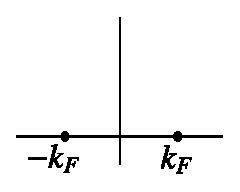
\includegraphics{images/lecture25/fig3a.eps}
\end{figure}

\section*{One dimension}

Fermi volume $=2k_{F}$
\begin{align*}
\therefore\quad N &= \frac{L}{2\pi}\cdot 2k_{F}=\frac{L}{2\pi}\cdot x\cdot \sqrt{\frac{2m}{\hbar^{2}}}\sqrt{E_{F}}=\sqrt{\dfrac{2m}{\hbar^{2}\pi^{2}}}\cdot \sqrt{E_{F}}\\
\therefore\quad D(E) &= \dfrac{dN}{dE}=\text{ const. } \sum\limits_{i}(E-\epsilon_{i})^{\frac{1}{2}}
\end{align*}
\begin{figure}[H]
\centering
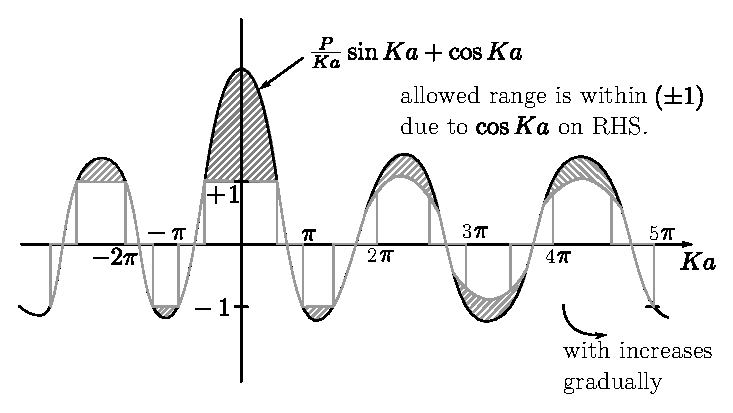
\includegraphics[scale=.8]{images/lecture25/fig3.eps}
\end{figure}

\section*{Two Dimension}

Formi volume $=\pi k^{2}_{F}=\dfrac{2m E_{F}}{\hbar^{2}}$
$$
\therefore\quad D(E)=\dfrac{dN}{dE}\simeq \text{ Const.}
$$
\begin{figure}[H]
\centering
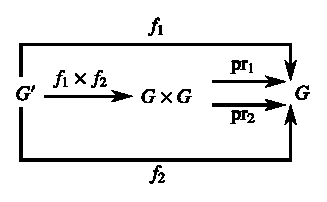
\includegraphics[scale=.8]{images/lecture25/fig4.eps}
\end{figure}

\section*{Three dimension}

Fermi volume $=\dfrac{4}{3}\pi k^{3}_F{}=\dfrac{4\pi}{3}\left(\sqrt{\dfrac{2mE_{F}}{\hbar^{2}}}\right)^{3}$
$$
\therefore\quad D(E)\sim \sqrt{E}
$$
\begin{figure}[H]
\centering
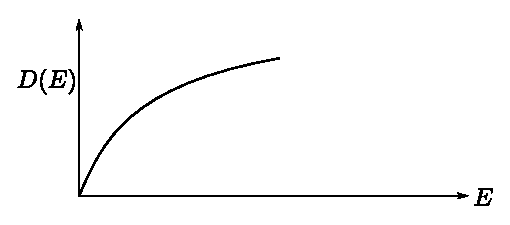
\includegraphics[scale=.8]{images/lecture25/fig5.eps}
\end{figure}

\noindent
{\bf Zero Dimension :- } Atomic levels like.

\noindent
{\bf Absorption :-}

\section*{Drude's model}

no. of electron per unit volume
$$
n=\dfrac{N}{V}\sim 6.02\times 10^{23}\dfrac{z\rho m}{A}
$$
\begin{quote}
$Z=$ atomic no.

$\rho_{m}=$ mass density.

$A=$ Atomic mass.
\end{quote}

Conduction electron density is a fraction of $n$ usually $n_{e}\sim 10^{22}/em^{3}$.

If $r_{S}$ is the radius of the volume per conduction electron
\begin{align*}
\therefore\quad \dfrac{V}{N} &=\dfrac{1}{n_{e}}=\frac{4}{3}\pi r^{3}_{S}\\
\therefore\quad r_{S} &= \left(\dfrac{3}{4\pi n_{e}}\right)^{\frac{1}{3}}
\end{align*}
$\dfrac{r_{S}}{a_{0}}\sim 2-3$ in most cases.

$a_{0}=$ Bohr radius.

$\simeq \dfrac{\hbar^{2}}{me^{2}}=0.529\times 10^{-8}$ cm.

In alkali metals $\dfrac{r_{S}}{a_{0}}\Rightarrow 3-6$

In some cases it can go upto $10$.

These are typically 1000 times greater than classical gas at NTP.

There can be strong electron-electron and electron ion interactions $\to$ still, in this model, we assume.
\begin{itemize}
\item[(i)] No. interaction between two collisions
\begin{itemize}
\item[(a)] Neglect of electron - electron interaction

$\to$ Independent electron approximation.

\item[(b)] Neglect of electron - ion interaction

$\to$ free electron approximation.
\end{itemize}
(a) often works well in real system but (b) is no good.

\item[(ii)] Collision of electrons with impenetrable ion core. Drude did not consider electron, electron scattering.

$\to$ One can simply talk about scattering effect without going into the detailed origin of scattering.

\item[(iii)] Probability of collision in a time duration, $dt\sim \dfrac{dt}{\tau}$, $\tau=$ relaxation time.

$\tau$ is independent of electrons position and velocity, it turns out that this approximation works well.

\item[(iv)] electrons achieve thermal equillibrium via collisions $\to$ Thermodynamic equillibrium via collisions.
\end{itemize}

\section*{DC Conductivity}

Ohm's law - $V=IR$

$\to E=\rho j$\quad $j=$ current density, $\rho=$ resistivity, $E=$ electric field.

$j=-neV$

$n\to$ electron density per unit volume.

$\nu\to$ average velocity.
\begin{figure}[H]
\centering
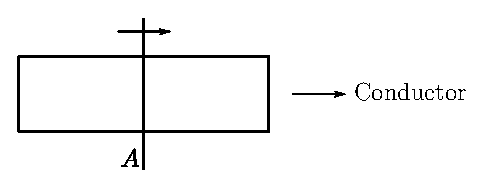
\includegraphics[scale=.8]{images/lecture25/fig6.eps}
\end{figure}

Random motion does not contribute in current flow. So, after a collision, velocity gain due to electric field is
\begin{gather*}
m\dfrac{dv}{dt}=-eE\\
a, V=-\dfrac{eEt}{m}\to \nu_{\text{arg}}=-\dfrac{eE\tau}{m}
\end{gather*}
$\tau=$ relaxation time $=t_{\text{arg}}$.
$$
\therefore\quad J=\left(\dfrac{ne^{\nu}\tau}{m}\right)E
$$
$a$, $\sigma=$ conductivity $=\dfrac{ne^{2}\tau}{m}$\quad $\rho=\dfrac{1}{\sigma}=\dfrac{m}{ne^{2}\tau}$
$$
a,\quad \tau = \dfrac{m}{\rho ne^{2}}
$$
at $RT$, $\rho\sim\mu$ Ohm-cm $=10^{-18}$ stat ohm-cm (in atomic units)
$$
\therefore\quad \tau=\left(\dfrac{0.22}{\rho_{\mu}}\right)\left(\dfrac{r_{S}}{a_{0}}\right)^{3}\times 10^{-14}\text{sec.}
$$
$\rho_{m}$ in units of micro-ohm-cm.

at $RT$, $\tau=10^{-14}\text{sec}$ to $10^{-15}$ sec. $\sim Fs$.

$\lambda=\nu_{0}\tau$

assuming classical equipartition theorem
$$
\frac{1}{2}m\nu^{2}_{0}=\dfrac{3}{2}k_{B}T\to \nu_{0}\sim 10^{7}\text{ cm/sec.}
$$
$\therefore \ \lambda \sim 1$ to $10\pi^{0}$.

In real materials. $\nu_{0}$ is an order of magnitude smaller and temperature independent.

$\tau$ at low temperature is an order of magnitude langer than the value at $RT$.

$\lambda$ is about $10^{3}$ times larger $\to$ much larger than lattice spacings.

At sufficiently low temperature $\lambda\sim\text{ cm}$.

$\therefore$ Bumping at ions seems not correct.

\section*{Tight binding model}

Free electron and nearly free electron picture gives good overview of the electronic structure in a solid and their properties.
\begin{itemize}
\itemsep=0pt
\item[$\to$] Quasi continuous distribution of energies with a gap in between.

\item[$\to$] For an improved description, one can start with atomic states by constructing a Block wave function through a {\em linear combination of atomic orbitals} (LCAO) 

This is called tight binding approximation.

\item[$\to$] Nearly free electron approx works for metals.

\item[$\to$] For covalently bonded solid or metals with localized electrons ($d$ and $f$), tight binding model is a better starting point.
\end{itemize} 

Lets start with the simplest form $\to$
$$
H_{at}=-\dfrac{\hbar^{2}\nabla^{2}}{2m}+V_{at}(r)\quad\text{for an atom.}
$$

Eigenvalues $E_{n}$ Eigen functions $\phi_{n}(r)$

For a Solid $\to$
\begin{align*}
H &= -\dfrac{\hbar^{2}\nabla^{2}}{2m}+\sum\limits_{R}V_{at}(r-R)\\[4pt]
  &= -\dfrac{\hbar^{2}\nabla^{2}}{2m}+V_{at}(r)+\sum\limits_{R\neq 0}V_{at}(r-R)\\[4pt]
  &= -\dfrac{\hbar^{2}\nabla^{2}}{2m}+V_{at}(r)+\nu(r)\\[4pt]
\nu(r)&=\sum\limits_{R\neq 0}V_{at}(r-R)
\end{align*}
non-local contribution.

If the atoms are places far away from each other, the atomic wave functions may be a good starting point.
\begin{align*}
\therefore\quad & \int \phi^{*}_{n}(r)H\phi_{n}(r)dr\\[4pt]
& =E_{n}+\int\phi^{*}_{n}\nu(r)\phi_{n}dr=E_{n}-\beta
\end{align*}
Small shift in energy due to other atoms becomes significant when $\nu(r)$ is appreciably large.

Now lets take a Bloch state to solve this problem.
$$
\psi_{k}(r)=\dfrac{1}{\sqrt{N}}\sum\limits_{R}e^{ik\cdot R}\phi_{n}(r-R)
$$
$\dfrac{1}{\sqrt{N}}$ is a normalization factor.
\begin{align*}
\therefore\quad E(k) &= \int \psi^{*}_{k}(r)H\psi_{k}(r)dr\\[4pt]
&= \int \sum\limits_{R,R'}\dfrac{1}{N}e^{ik(R-R')}\phi^{*}_{n}(r-R)H\phi_{n}(r-R)dr
\end{align*}

\newpage

All sums for a particular choice of $R'$ should be same as long as translational symmetry is preserved.
\begin{align*}
\sum\limits_{R'}f &= Nf(R'=0)\\[4pt]
\therefore\quad E(k) &= \sum\limits_{R}\int \phi^{*}_{n}(r)H\phi_{n}(r-R)dr\\[4pt]
&= E_{n}-\beta+\sum\limits_{R\neq 0}\int \phi^{*}_{n}(r)H\phi_{n}(r-R) dr\\[4pt]
I &= E_{n}\int\phi^{*}_{n}(r)\phi_{n}(r-R)dr+\sum\limits_{R\neq 0}\int \phi^{*}_{n}(r)\nu(r)\phi_{n}(r-R)dr
\end{align*}
$0$ as $\phi$'s are centered at two different atoms.

`$X$' is also close to zero, but can be appreciable if $\nu(r)$ becomes large when approaching the neighbor.
\begin{gather*}
\to `X' = -\gamma(R)\\
\therefore\quad E(k)=E_{n}-\beta-\sum\limits_{R\neq 0}\gamma(R)e^{ik.R}
\end{gather*}
for an one dimensional solid, considering only nearest neighbors.
$$
E(k)=E_{n}-\beta-\gamma(e^{ika}+e^{-ika})=E_{n}-\beta-2\gamma \cos ka
$$
\begin{figure}[H]
\centering
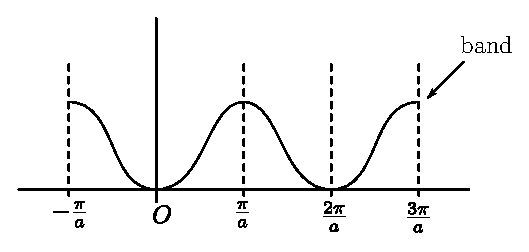
\includegraphics[scale=.8]{images/lecture25/fig7.eps}
\end{figure}
One can calculate the band structure for $s$-band, $p$-band etc.
\begin{figure}[H]
\centering
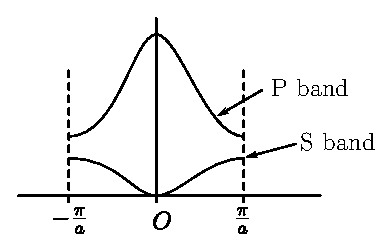
\includegraphics[scale=.8]{images/lecture25/fig8.eps}
\end{figure}
General form of tight binding Hamiltonian.
$$
H=\sum\limits_{i}\epsilon_{i}a_{i}^{t}a_{i}+\sum\limits_{i>j}t_{ij}a_{j}^{t}a_{i}\quad t_{ij}=\langle J |H|i\rangle
$$
If one includes electron-electron coulomb repulsion then if becomes the Hubbard Hamiltonian.
$$
H=\sum t_{ij}a^{t}_{j}a_{i}+\sum_{\alpha\beta}U_{\alpha\beta}n_{\alpha}n_{\beta}\sum_{ijkl}U_{ijkl}a_{i}^{t}a^{t}_{j}a_{k}a_{l}
$$
$\epsilon$'s are neglected as it gives a constant shift in energy $\to$ change in reference energy.

\section*{Magnetism}

Gauss' law for magneto statics $\oint B\cdot da=0$ \ $\overrightarrow{\nabla}\cdot \overrightarrow{B}=0$ as there are no magnetic monopole.

Source of magnetic induction is magnetic dipole
\begin{align*}
\overrightarrow{B}=\mu_{0}H\quad \mu_{0} &= \text{permeability}\\
&= 4\pi \times 10^{-7}V_{S}\overrightarrow{A}^{1}m^{-1}\\
&= 4\pi \times 10^{-7}T^{2}m^{3}T^{-1}
\end{align*}
SI unit of $B$ is Tesla $=kg5^{2}A^{-1}$.

Earth's magnetic field
$$
\sim 0.25-0.65 G= 2.5\times 10^{-5}-6.5\times 10^{-5}\text{~ Tesla.}
$$

In matter $\to B=\mu_{0}(H+M)=B_{0}\text{ (applied field)} + \mu_{0}M\text{ (magnetization)}$

If $N=$ No. of dipole moments, $\mu$ in a volume, $V$ 

$M=\mu\dfrac{N}{V}$ and is related to applied field $B$. One can write $\mu_{0}M=\chi_{m}B_{0}$, $\chi_{m}=$ magnetic susceptibility.
\begin{align*}
\chi_{m} \to & \text{-ve system is called diamagnetic}\\
            & \text{+ve it is called paramagnetic}
\end{align*}
$\therefore \ \mu=1+\chi_{m}=$ relative permeability $\Leftarrow \fbox{$B=\mu_{0}\mu B_{0}$}$

Note: This should not be confused with magnetic moment $\mu$. We normally don't use this term, instead describe in terms of $\chi$.

Assumption $\to$ linear relation, in Ferromagnet, $\mu$ depends on hystory of the test material.

Potential energy of a magnetic dipole is $V=-\overrightarrow{\mu}B_{0}$, $\overrightarrow{\mu}=$ magnetic moment.

Since, $M$ depends on field, one cannot write $U=-V\overrightarrow{M}\cdot \overrightarrow{B}_{0}$ as system energy
\begin{align*}
\therefore\quad U &= -V\int\limits^{B_{0}}_{0}Mdb'_{0}\\
&= -\dfrac{VX_{m}}{\mu_{0}}\int\limits^{B_{0}}_{0}B'_{0}dB'_{0}=-\dfrac{VX_{m}}{2\mu_{0}}B^{2}_{0}
\end{align*}
Since, $\overrightarrow{B}$ and $\overrightarrow{M}$ are usually parallel we can ignore vector expressions.

$U$ becomes more (-ve) with increase in $B_{0}$.

$\therefore \ \overrightarrow{\mu}$ experience a force towards the direction of field in paramagnets $\to$ towards the location of the field.

For diamagnets, it goes away from the regions of high magnetic field as $x_{m}$ is (-vi).

{\bf Lenz's law - } magnetic moment arising from the motion of electrons due to external magnetic field opposes the external field $\to$ diamagnetism.

Closed shell configuration $\to$ diamagnetism, it is always there in any magnetic system.

Paramagnetism appears when there is net magnetic moment. in such cases diamagnetism is not visible as the effect due by fimit moments dominate the magnetism.

While diamagnetism may be captured in some way using such classical picture but atom cannot have magnetic moment in such descriptions $\to$ {\em Bohr - Van Lecuwen theorem.}

\noindent
{\bf Quantum picture $\to$}
$$
B=\nabla \times A \text{ \ vector potential}
$$

$\therefore$ In presence of magnetic field $p\to p-\dfrac{qA}{c}$
$$
A=\dfrac{1}{2}\overrightarrow{r}\times \overrightarrow{B}\quad q=\text{charge}
$$
\begin{align*}
\dfrac{P^{2}}{2mc} &\Rightarrow \dfrac{1}{2m_{e}}(p+eA)^{2}=\dfrac{1}{2}m_{e}\left(p-e\dfrac{r\times B}{2}\right)^{2}\\
&= \frac{1}{2m_{e}}\left(p^{2}+eB_{0}(r\times p)+\dfrac{e^{2}}{4}(r\times B_{0})^{2}\right)
\end{align*}
For $B=B_{z}$
\begin{align*}
H &= H_{0}+H'\Rightarrow H'=\dfrac{e}{2m_{e}}B_{0}(r\times P)_{z}+\dfrac{B^{2}}{8m_{e}}B^{2}_{0}(x^{2}+y^{2})\\
\therefore\quad E' &= \dfrac{e}{2m_{e}}B_{0}\langle \psi|r\times P|\psi\rangle +\dfrac{e^{2}}{8m_{e}}B^{2}_{0}<\psi |x^{2}\times y^{2}|\psi\rangle
\end{align*}
Orbital momentum.

Paramagnetic term. For an electron, it is negative and becomes more negative for higher $B_{0} \to$ moments align along the field to lower its energy.

always positive energy increases with increase in $B\to$ diamagnetic term.


Electron has a spin momentum $\to$ Comes from relativistic QM. So we need to add that term here too.

Orbital term $\to \ \dfrac{e}{2m_{e}}B_{0}\langle \psi |r\times p|\psi\rangle =\mu_{B}\cdot m_{t}B_{0}$

$m_{C}=$ orbital angular moment.

Spin term $\to g_{e}m_{S}\dfrac{e\hbar}{2m_{e}}B_{0}=g_{e}m_{S}\mu_{B}B_{0}\mu_{B}=\dfrac{e\hbar}{2m_{e}}=$ Bohr magnetic.
\begin{align*}
m_{S} &= \text{spin magnetic moment }=9.274\times 10^{-24}\text{ Joule } T^{-1}\\
&= \pm \dfrac{1}{2}=5.788\times 10^{-5}eVT^{-1}\\
g_{e} &\approx 2 = \text{gyromagnetic ratio.}
\end{align*}
In an atom, magnetic field leads of precesion of the orbital and spin - moments.

Due to orbital moment
\begin{align*}
\mu &= -\dfrac{e\hbar}{2m_{e}}L=-\mu_{B}L\\
&= -m_{l}\mu_{B}
\end{align*}
$L\to$ orbital angular momentum.

$m_{e}$ takes values $-l,\ldots,0,\ldots+l=(2l+1)\text{ values}$.

If $J$ is the total angular momentum, then one can define 
$$
\mu_{J}=-gm_{J}\mu_{B}\quad g\to \text{Lande `$g$' factor.}
$$
$m_{J}$ take $(2J+1)$ values.

For light atoms, spin-orbit coupling is weak, so one can calculate $J$ by summing total orbital and spin-moments separately $\to$ L-S Coupling or Russel Sanders Coupling.
$$
L=\sum m_{l}\quad S=\sum m_{S}
$$
To get the lowest energy configuration, one can use {\em Hund's rule}.
\begin{itemize}
\item[(i)] Maximum $S$ consistent with Pauli principle, has the lowest energy.

\item[(ii)] For a given $S_{1}$ maximum value of $L$ has the lowest energy.

\item[(iii)] For a shell less than half filled $J=L-S$
\begin{center}
\begin{tabular}{rl}
 & for more than half filled $J=L+S$\\
 & $J-S$ for half filled case, here, $L=0$\\
 & $3J(J+1)+S(S+1)-L(L+1)$\\
\cline{2-2}
$g_{J}=$ & \multicolumn{1}{c}{$2J(J+1)$}
\end{tabular}
\end{center}
\end{itemize}
\begin{itemize}
\item[$\to$] Open shell configuration gives magnetic moment.

\item[$\to$] Electron correlation is important to have magnetic moment
\end{itemize}
for moment aligned along $B$.

We know $\mu=gJ\mu_{B}$ and Energy = $-g\mu_{B}JB_{0}$ using Boltzmann distance.

mean moment at a temperature $T$ is
\begin{align*}
\overline{\mu} &= \frac{1}{z}\sum\limits^{+J}_{m_{j}=-J}g_{J}\mu_{B}m_{J}e^{(g_{J}\mu_{B}m_{J}B_{0}/k_{B^{T}})}\\
z &= \text{ partition function } = \sum e^{g_{J}\mu_{B}m_{J}B_{0}/k_{B^{T}}}
\end{align*}
\begin{itemize}
\item[(i)] Foe $g_{J}\mu_{B}B_{0}\gg k_{B^{T}}$ field is strong enough to align all the moments.

$\mu$ saturates, But it is hard to realize this experimentally as thermal fluctuations are strong.

\item[(ii)] $g_{J}\mu_{B}B_{0}\ll k_{B^{T}}\Rightarrow \fbox{$X_{m}=\dfrac{M}{H}=\dfrac{C}{T}$}$ Curie's law.
$$
C=\dfrac{\mu_{0}Ng^{2}_{J}\mu^{2}_{B}J(J+1)}{3Vk_{B}}
$$
\begin{figure}[H]
\centering
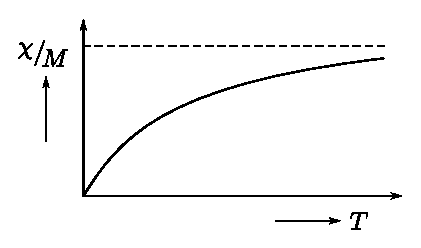
\includegraphics[scale=.8]{images/lecture25/fig9.eps}
\end{figure}
\end{itemize}
These values woks well for rare earths. But for 3d elements, it is not good due to quenching of orbital moment $\to$ orbitals are exposed to crystal field $\to$ orbital moment is not a good quantum no. 

{\bf Pauli paramagnetism} $\to$ Paramagnetism due to conduction electrons.
\begin{figure}[H]
\centering
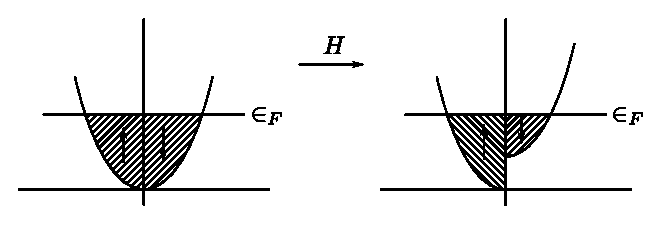
\includegraphics[scale=.8]{images/lecture25/fig10.eps}
\end{figure}

\noindent
{\bf Exchange interation = \boldmath$X$}
$$
H=-\sum\limits_{i\neq J}X_{ij}S_{i}\cdot S_{j} \text{ (Heisenberg term) }+g_{e}\mu_{B}B_{0}\cdot \sum\limits_{i}S_{i}
$$

\noindent
{\bf Nobel Prize in Chemistry, 1998} to {\em Walter Kohn} for his development of the density functional theory and {\em John Pople} for his development of computational methods in quantum chemistry.

The large intensity of the ultraviolet beam in the UPS measurements makes it difficult to neutralize the intense charging effect. In the BIS measurements an intense negative charging arises due to the electron beam impinging on the surface; there is no reliable way to take care of such charging effects. Thus, in the highly insulting samples it was not possible to perform the UPS and BIS measurements.

\section*{B. Theoretical methods}

\section*{2.4 Band structure calculation : LMTO -ASA}

Electronic band structures for all the systems discussed in this thesis were calculated using Linearized-Muffin-Tin Orbital method within the Atomic Sphere Approximations (LMTO-ASA). An exhaustive description of this method can be found elsewhere [14]. Here, we point out the basic formalism in brief with a mention of the various approximations. The Hamiltonian of a system of $N$ electrons in a lattice is given by,
\begin{equation*}
H=\sum\limits^{N}_{i}(-\nabla^{2}_{i})+\frac{1}{2}\sum\limits^{N}_{i,j;i\neq j}\dfrac{2}{r_{ij}}+\sum\limits^{N}_{i}v_{ext}(r_{i})=T+V_{ee}+V_{ext}\tag{2.10}
\end{equation*}
where the first term $(T)$ represents the kinetic energy, second term $(V_{ee})$ is the electron Coulomb repulsion and the last term $(V_{ext})$ is the interaction with the external potential, which includes the electrostatic interaction with the fixed nuclei. According to {\em Hohenberg and Kohn's theorem} [15]; (i) the external potential is a unique functional of the electron density $n(r)$ and (ii) the energy functional assumes its minimum value, the ground state energy, for the correct ground state density. Using these theorems the Hamiltonian can be solved. In the case of non-interacting system, the Hamiltonian reduces to,
\begin{equation*}
H=T+V_{ext}=\sum\limits^{N}_{i}(-\nabla^{2}_{i})+\sum\limits^{N}_{i}v_{s}(r_{i}), \text{ Kohn-Sham potential.}
\end{equation*}
where $v_{s}(r_{i})$ is the effective single particle potential and the ground state wave function in this problem is {\em a Slater determinant obtained by populating the lowest-lying one-electron orbitals defined by the Schr\"odinger equation},
$$
H\psi_{i}(r)=E_{i}\psi_{i}(r)\to \text{ Kohn-Sham equation}
$$
Kohn-Sham wave function $\to$ Single Slater determinant constructed from a set of orbitals that are lowest energy solution of $H\psi=E\psi$.

Kohn-Sham potential $\to$ Effective external potential, in which non-interacting particles move and the density function can be represented as,
\begin{equation*}
n(r)=\sum\limits^{occ}_{j}|\psi_{j}(r)|^{2}\tag{2.13}
\end{equation*}
In order to obtain a solution for the real systems Kohn and Sham [16] adopted the non-interacting density functions to the interacting ones. In this description the kinetic energy is in terms of the non-interacting wave function and can be expressed as,
\begin{equation*}
\langle T\rangle =\sum\limits^{occ}_{j}\int\psi^{*}_{j}(r)(-\nabla^{2})\psi_{j}(r)dr\tag{2.14}
\end{equation*}
and the electron-electron interaction energy is considered to be a combination of a Hartree term and an exchange term,
\begin{equation*}
E_{ee}=\dfrac{1}{2}\int \dfrac{2n(r)n(r')}{|r-r'|}drdr'+E_{xc}[n]\tag{2.15}
\end{equation*}
$E_{xc}[n]$ is the exchange-correlation energy functional. In order to evaluate this energy, calculations incorporate a local density approximation (LDA) where
\begin{equation*}
E_{xc}[n]=\int \epsilon_{xc}(n(r))n(r)dr\tag{2.16}
\end{equation*}
Thus, the fluctuations in the density functionals are neglected in this calculation. These approximations results in the effective single particle potential function given by,
\begin{equation*}
V_{s}(r)=\int \dfrac{2n(r')}{|r-r'|}dr'+v_{ext}(r)+v_{xe}(n(r))\tag{2.17}
\end{equation*}
where,
\begin{equation*}
v_{xc}(r)=d(n\epsilon_{xc}(n))/dn\tag{2.18}
\end{equation*}
The above formalism does not treat the spin contributions separately. In order to obtain the magnetic properties of the systems, the density functional formalism has been extended to spin-density formalism, known as local spin density approximation (LSDA), where the spin up and spin down densities, $n_{\uparrow}(r)$ $n_{\downarrow}(r)$ are treated as independent variables. In terms of these variables the electron density $(n(r))$ and magnetization density $(m(r))$ are expressed as,
\begin{align*}
n(r) &= n_{\uparrow} (r)+n_{\downarrow}(r)\tag{2.19}\\
m(r) &= n_{\uparrow} (r)-n_{\downarrow}(r)\tag{2.20}
\end{align*}
and the exchange term in the potential function becomes a function of $n_{\uparrow}(r)$ and $n_{\downarrow}(r)$. 

The ground state electron-spin density is determined by a self consistent procedure using the single particle Schr\"odinger equation,
\begin{equation*}
H\psi_{i\sigma}=E\psi_{i\sigma} \ ; \ H=-\nabla^{2}+V_{s}(r)\tag{2.21}\label{lec25-eq2.21}
\end{equation*}
where $\sigma$ denotes the spin of the system; the spin densities and $V_{s}(T)$ are
\begin{equation*}
n_{\sigma}(r)=\sum\limits^{occ}_{i}|\psi_{i\sigma}(r)|^{2}\tag{2.22}\label{lec25-eq2.22}
\end{equation*}
and
\begin{equation*}
V_{s}(r)=\int \dfrac{2m(r')}{|r-r'|}dr'+v_{ext}(r)+v_{xc}(n_{\uparrow}(r),n_{\downarrow}(r))\tag{2.23}\label{lec25-eq2.23}
\end{equation*}
The equations \eqref{lec25-eq2.21} and \eqref{lec25-eq2.22} are interdependent and thus solved self-consistently. The equation \eqref{lec25-eq2.21} is known as the Kohn-Sham equation and provides a mathematical way to arrive the ground state solution self-consistently [17]. The Kohn-Sham eigen energy, $\epsilon_{i\sigma}$, is related to the total energy in terms of the infinitesimal variation of the occupation number of the eigen-state, $\delta n_{i\sigma}$;
\begin{equation*}
\delta E_{tot}=\sum\limits_{i\sigma}\epsilon_{i\sigma}\delta n_{i\sigma}\label{lec25-eq2.24}
\end{equation*}
Since infinitesimal part of an electron is not a physical object, the energy obtained from the above relation is not a physically observable quantity. However, in practice, the Kohn-Sham eigen energies, $\epsilon_{i\sigma}$ often observed to provide a good approximation of the quasiparticle energy, except for the energy band gap [18, 19].

LMTO = Muffin-tin orbital method.

LAPW = Augmented plane wave method.

Pseudopotential method.

OPW = Orthogonalized plane wave method.

There are many ways of solving the above equations with or without the spin polarizations. Our calculations involve the LMTO-ASA method to solve the problem. In LMTO method, the solid has been assumed to be a network of atomic spheres, called muffin-tin orbitals (MTO) are regular, continuous and differentiable everywhere. Within the muffin-tin spheres, these orbitals are constructed from the partial waves $\psi_{l}(E^{l}_{v},r)$ and their first energy derivatives, $\partial\psi_{l}(E^{l}_{v},r)/\partial E^{l}_{v}|_{E=E^{l}_{v}}$ evaluated at a fixed but arbitrary energy $E^{l}_{v}$. Outside the sphere MTO is a partial wave of fixed energy. Thus, the problem can be solved using various conventional self-consistent methods. However, the solution can be achieved much faster by reducing it to an eigenvalue problem with the linear combination of muffin-tin orbitals as the eigenfunctions and treating the Hamiltonian in a variational procedure. The linearization of the basis functions reduces the calculational complexity, but the energy eigenvalues are accurate only in a certain energy region close to $E^{l}_{v}$. The value of $E^{l}_{v}$ is normally chosen as the center of gravity of the occupied part of the corresponding partial density of states (PDOS) for the ground state calculation. Here the PDOS are the density of states (DOS) projected on the basis functions used for the calculations. $s$, $p$, $d$ and sometimes $f$ states were used as basis functions in the calculations.

A further simplification in the problem is achieved by introducing the atomic sphere approximation (ASA). In this case the volume of the atomic spheres are assumed such that the total volume arising from all the spheres in the unit cell is equal to the unit cell volume. In crystal structures not so closely packed, this may necessitate the introduction of empty spheres with no charge within the spheres and the positions satisfying the symmetry of the real lattice. This volume filling criterion leads to a partial overlap of the atomic spheres. Moreover, the kinetic energy is taken to be zero at the interstitial region, as a consequence of which, the basis functions in the interstitial region are solutions of the Laplace equation. Such drastic approximations involved in ASA leads to inaccuracies in the effect of nearest neighbor orbitals. A combined correction term has been included in the calculation which helps in partial re-establishment of the kinetic energy at the interstitials and also corrects for the neglect of the higher partial waves.

The linearization about the $E^{l}_{v}$ provide reasonable description of the density of states in the occupied part; the same results are also used to calculate the spectral functions for the unoccupied part. It is observed that the calculated results often do not produce the unoccupied part. In order to avoid problems due to linearization, calculations were also performed with converged potential parameters from a regular self-consistent calculation, but with the $E^{l}_{v}$'s shifted towards higher energies. Some of the results are presented by contracting the energy scale of the spectral function obtained from the normal self-consistent procedure for the unoccupied part. Such processes are found to be reasonably successful in describing the BI and XA spectra [20].
